% document formatting
\documentclass[10pt]{article}
\usepackage[utf8]{inputenc}
\usepackage[left=1in,right=1in,top=1in,bottom=1in]{geometry}
\usepackage[T1]{fontenc}
\usepackage{xcolor}

% math symbols, etc.
\usepackage{amsmath, amsfonts, amssymb, amsthm}
\usepackage{dsfont}

% lists
\usepackage{enumerate}

% images
\usepackage{graphicx} % for images
\usepackage{tikz}
\usetikzlibrary{fit}

% code blocks
\usepackage{minted, listings} 

% verbatim greek
\usepackage{alphabeta}
\DeclareMathOperator*{\argmin}{arg\,min}
\DeclareMathOperator*{\argmax}{arg\,max}

\graphicspath{{./assets/images/}}

\title{02-750 Week 3 \\ \large{Automation of Scientific Research}}
 
\author{Aidan Jan}

\date{\today}

\begin{document}
\maketitle

\section*{Artificial Intelligence}
Note that machine learning is a subset of artificial intelligence.  Deep learning is a subset of machine learning.

\subsection*{What is Artificial Intelligence (AI)?}
``Any task performed by a machine that would have previously been considered to require human intelligence.'' - Professors Mavin Minsky and John McCarthy (1956)
\begin{itemize}
	\item ``It is the science and engineering of making intelligent machines, especially intelligent computer programs.  It is related to the similar task of using computers to understand human intelligence, but AI does not have to confine itself to methods that are biologically observable.'' - Professor John McCarthy (2004)
	\item ``A system's ability to adapt and improvise in a new environment, to generalize its knowledge and apply it to unfamiliar scenarios.'' - AI researcher Fran\c{c}ais (2020)
\end{itemize}

\subsection*{What is Machine Learning (ML)?}
\begin{itemize}
	\item A branch of AI
	\item ``Study of computer \textbf{algorithms} that allow computer programs to automatically \textbf{improve} through \textbf{experience}.'' - Prof. Tom Mitchell (1997)
\end{itemize}
\begin{center} 
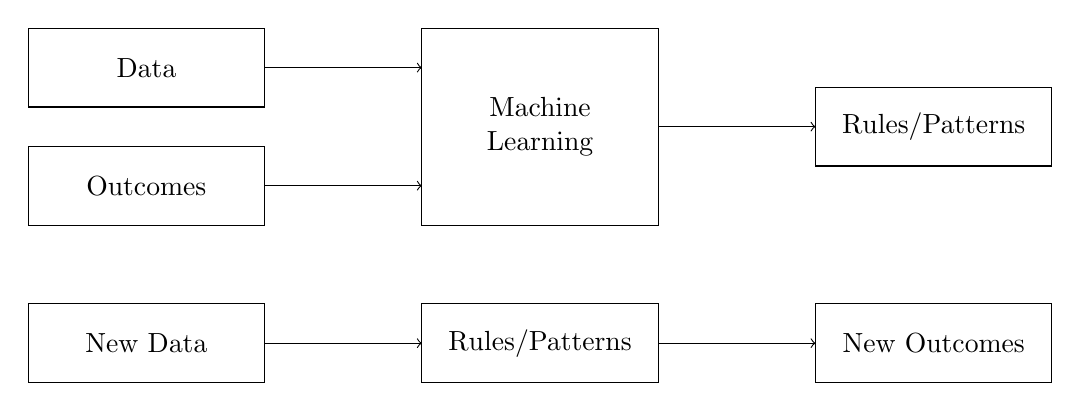
\begin{tikzpicture}
    \draw (0, 4) rectangle (3, 3) node[midway] {Data};
    \draw (0, 2.5) rectangle (3, 1.5) node[midway] {Outcomes};
    \draw (5, 4) rectangle (8, 1.5) node[midway, align=center] {Machine\\Learning};
    \draw (10, 3.25) rectangle (13, 2.25) node[midway] {Rules/Patterns};

    \draw (0, 0.5) rectangle (3, -0.5) node[midway] {New Data};
    \draw (5, 0.5) rectangle (8, -0.5) node[midway] {Rules/Patterns};
    \draw (10, 0.5) rectangle (13, -0.5) node[midway] {New Outcomes};
    
    \draw[->] (3, 3.5) -- (5, 3.5);
    \draw[->] (3, 2) -- (5, 2);
    \draw[->] (8, 2.75) -- (10, 2.75);
    \draw[->] (3, 0) -- (5, 0);
    \draw[->] (8, 0) -- (10, 0);
\end{tikzpicture}
\end{center}

\subsection*{Types of Machine Learning}
\begin{itemize}
	\item Supervised Learning
	\begin{itemize}
	    \item Input: Training data and labels.
	    \item Goal: Learn function to map new unlabelled data to labels.
	    \item For example, classification and regression.
    \end{itemize}
	\item Semi-Supervised Learning
	\begin{itemize}
	    \item Input: Training data, some of which is labelled.
	    \item Goal: Learn function to map new unlabelled data to labels and/or learn structure in the data.
    \end{itemize}
	\item Reinforcement Learning
	\begin{itemize}
	    \item Given a sequence of states and actions with (delayed) rewards, output a policy
	    \item Policy is a mapping from states to actions that tells you what to do in a given state.
	    \item Agent and environment interact at discrete time steps.  Agent commits ana action on the environment, which changes its state and rewards (either positively or negatively) the agent.
	    \item For example, training a self-driving car.
    \end{itemize}
	\item Unsupervised Learning
	\begin{itemize}
	    \item Input: Training data without labels.
	    \item Goal: Learn structure in the data.
	    \item For example, K-means Clustering
    \end{itemize}
\end{itemize}

\subsection*{When to Use Machine Learning}
Machine Learning is used when:
\begin{itemize}
	\item human expertise does not exist (e.g., navigating on Mars)
	\item humans can't explain their expertise (e.g., speech recognition)
	\item models must be customized (e.g., personalized medicine)
	\item models are based on huge amounts of data (e.g., genomics)
\end{itemize}
Learning isn't always useful:
\begin{itemize}
	\item There is no need to "learn" to calculate payroll
\end{itemize}

\subsection*{Designing a Learning System}
\begin{itemize}
	\item Choose the training experience
	\item Choose exactly what is to be learned (i.e., the \textit{target function})
	\item Choose how to represent the target function
	\item Choose a learning algorithm to infer the target function from the experience
\end{itemize}

\subsection*{Training vs. Test Distribution}
\begin{itemize}
	\item We generally assume that the training and test examples are independently drawn from the same overall distribution of data
	\begin{itemize}
	    \item We call this ``i.i.d'' which stands for ``independent and identically distributed''
    \end{itemize}
    \item If examples are not independent, it requires \textit{collective classification}.
    \item If the test distribution is different, it requires \textit{transfer learning}.
\end{itemize}

\subsection*{ML in a Nutshell}
\begin{itemize}
	\item Tens of thousands of machine learning algorithms.  (Hundreds of new ones every year)
	\item Every ML algorithm has three components:
	\begin{itemize}
	    \item Representation
	    \item Optimization
	    \item Evaluation
    \end{itemize}
    \item Deep Learning tends to do better than most machine learning algorithms when the amount of data grows large.
\end{itemize}

\subsection*{Various Function Representations}
\begin{itemize}
	\item Numerical functions
	\begin{itemize}
	    \item Linear Regression
	    \item Neural Networks
	    \item Support Vector Machines
    \end{itemize}
    \item Symbolic functions
    \begin{itemize}
	    \item Decision trees
	    \item Rules in propositional logic
	    \item Rules in first-order predicate logic
    \end{itemize}
    \item Instance-based functions
    \begin{itemize}
	    \item Nearest-neighbor
	    \item Case-based
    \end{itemize}
    \item Probabilistic Graphical Models
    \begin{itemize}
	    \item Na\text{\"i}ve Bayes
	    \item Bayesian networks
	    \item Hidden-Markov Models (HMMs)
	    \item Probabilistic Context Free Grammars (PCFGs)
	    \item Markov networks
    \end{itemize}
\end{itemize}

\subsection*{Various Search / Optimization Algorithms}
\begin{itemize}
	\item Gradient Descent
	\begin{itemize}
	    \item Perceptrons
	    \item Backpropagation
    \end{itemize}
	\item Dynamic Programming
	\begin{itemize}
	    \item HMM Learning
	    \item PCFG Learning
    \end{itemize}
	\item Divide and Conquer
	\begin{itemize}
	    \item Decision tree induction
	    \item Rule learning
    \end{itemize}
	\item Evolutionary Computation
	\begin{itemize}
	    \item Genetic Algorithms (GAs)
	    \item Genetic Programming (GP)
	    \item Neuro-evolution
    \end{itemize}
\end{itemize}

\subsection*{Evaluating ML Models}
\begin{itemize}
	\item Accuracy
	\item Precision and Recall
	\item Squared Error
	\item Likelihood
	\item Posterior Probability
	\item Cost / Utility
	\item Margin
	\item Entropy
	\item K-L Divergence
	\item etc.
\end{itemize}

\section*{Prototypical Active Learning Algorithm}
Obtain initial labeled training data $D_L = \{(x_1, y_1), \cdots, (x_n, y_n)\}$, where each $x_i \in \mathcal{X}$ is an input input and $y_i \in \mathfrak{C}$ its corresponding label.
\begin{itemize}
	\item Repeat, until we hit stopping criterion.  (Exit the loop when we run out of money or decide the model is good enough.)
	\begin{itemize}
	    \item Learn model: $h = Learn(D_L); h \in \mathcal{H}$.  This function is called the `Base Learner'; it can be any supervised learning algorithm.
	    \item Select the next point to label, $x_i \in \mathcal{X}$, according to the data access model.  This is the `Query selection' step.  The \textbf{data access model} determines which instances are selectable at any given time.
	    \item Pay ``oracle'' for $x_i$'s label, $y_i \in \mathfrak{C}$.  (The oracle tells us the true label of a selected instance, and is typically a wet lab experiment, a Ph.D. student, data scientists, etc.)
	    \item Update training data: $D_L = D_L \cup \{(x_i, y_i)\}$
    \end{itemize}
	\item Output final model: $h = Learn(D_L)$
\end{itemize}

\subsection*{Data Access Model}
Regardless of the data access model, queries are made based on the \textbf{expected utility} of each instance.  Informally, the utility of an instance is the degree to which it helps us improve the model.
\begin{center} 
	\includegraphics*[width=0.8\textwidth]{W3_1.png} 
\end{center}

\subsubsection*{Membership Query Synthesis (MQS)}
MQS selectors can request \textbf{any} point in $\mathcal{X}$ (i.e., instances space)
\begin{itemize}
	\item In science, $\mathcal{X}$ will often represent a space of possible experiments.
\end{itemize}
This setting includes queries that the learner generates \textit{de novo}, rather than those sampled from some underlying natural distribution.

\subsubsection*{Stream-based Selective Sampling}
Selective samplers are presented a stream of unlabeled instances
\begin{itemize}
	\item Examples: automated chemical synthesis and characterization; flow cytometry
\end{itemize}
Each unlabeled instance is drawn one at a time from the data source
\begin{itemize}
	\item The learner decides whether to request label, or not
	\item If no label is request, the instance is 'lost'
\end{itemize}
Stream-based selective sampling is less common in basic research because we \textbf{usually} preserve all the data and/or samples for future access.  Stream-based sampling is more relevant to engineering contexts, where the ultimate goal may be to iteratively improve an underlying design in real-time.

\subsubsection*{Pool-based Sampling}
Pool-based samplers have access to a large unlabeled pool $\mathcal{U}$.
\begin{itemize}
	\item Examples: tissue banks; electronic medical records; unlabeled images.
	\item Common in biological research when it is easy to obtain data (e.g., images) but it is costly to obtain labels.
\end{itemize}

\subsection*{Query Selection Methods}
\begin{itemize}
	\item There are many different approaches to query selection
	\item Some methods are merely \textit{heuristics}.  (i.e., they provide no formal guarantees)
	\item Others do come with one or more formal guarantees (i.e., we can prove theorems about them)
	\item For example, guarantees with respect to:
	\begin{itemize}
	    \item Sample complexity (the number of samples needed to learn a `good' model)
	    \item Statistical consistency (a guarantee that the model will converge to the 'true' model, given a sufficient amount of training data, even though it is not \textit{iid})
    \end{itemize}
\end{itemize}

\section*{Heuristic Query Selection Methods}
\subsection*{Uncertainty Sampling}
Generic uncertainty sampling algorithm (pool-based sampling)
\begin{verbatim}
Input U := a pool of unlabeled instances and D_L := labeled training data
Output h = learn(D_L)
for i = 1, 2, ... do
    h = Learn(D_L);
    Select x_i in U, the most uncertain instance according to model h
    Query the 'oracle' for x_i's label, y_i
    D_L += {(x_i, y_i)}
    Remove x_i from U
return h = Learn(D_L)
\end{verbatim}
Here, the notion of uncertainty is with respect to the model's confidence in $x$'s label.

\subsubsection*{Aside: Single vs. Batch Mode Learning}
In science, the fixed costs of obtaining labels (i.e., by running experiments) can sometimes be amortized over multiple queries.  For example, running 96 experiments at once in a 96-well plate.
\begin{itemize}
	\item When this is true, the query selection algorithm may be asked to select \textbf{batches} of queries for each round, instead of individual experiments.
	\item Batch-mode query selection is something that can, in principle, be added to most active learning algorithms
	\item Same algorithm as the one above, but instead of selecting one \texttt{x\_i}, we select the top $k$ most uncertain instances.
\end{itemize}

\subsubsection*{Quantifying Uncertainty: Probabilistic Classifiers}
\begin{itemize}
	\item Least Confident: $x_{LC}^* = \argmax_{x \in \mathcal{U}} 1 - P(\hat{y} | x)$.  Here, $\hat{y} = \argmax_{y \in \mathfrak{C}} P(y | x)$
	\item Smallest margin: $x_{M}^* = \argmin_{x \in \mathcal{U}} P(\hat{y}_1 | x) - P(\hat{y}_2 | x)$.  Here, $\hat{y}_1$ and $\hat{y}_2$ are the first and second most probable class labels, respectively.  Small margins mean it is difficult to distinguish between two most-likely labels.
	\item Entropy: $x_H^* = \argmax_{x \in \mathcal{U}} - \sum_{y \in \mathfrak{C}} P(y | x) \log P(y | x)$
	\begin{itemize}
	    \item Entropy is a measure over a probability distribution
	    \item Higher entropy means more uncertainty about the labels
	    \item Entropy is an information-theoretic measure that represents the amount of information needed to encode a distribution.
    \end{itemize}
\end{itemize}
Visualizing uncertainty (binary classification)
\begin{center} 
	\includegraphics*[width=0.8\textwidth]{W3_2.png} 
\end{center}
Visualizing uncertainty (ternary classification)
\begin{center} 
	\includegraphics*[width=0.8\textwidth]{W3_3.png} 
\end{center}
Here, color is proportional to uncertainty.  (Black is highest.)  Empirical comparisons of these measures suggest that the best strategy may be application-dependent.

[stop 49]

\subsection*{Query by Committee}

\subsection*{Expected Model Change}

\subsection*{Minimizing Expected Risk}

\subsection*{Density-based Sampling}


\section*{Heuristic Query Selection Methods}
\subsection*{Uncertainty Sampling}
\subsubsection*{Quantifying Uncertainty for Regression}
\begin{itemize}
	\item For regression problems, uncertainty is often quantified as the \textbf{output variance} (i.e., variance of the conditional distribution on $y$)
	\item Example: 1D regression model
\end{itemize}
\begin{center} 
	\includegraphics*[width=0.8\textwidth]{W3_4.png} 
\end{center}
Consider the predictions made by a simple linear regression model
\[Y = \beta_0 + \beta_1 x + \epsilon\]
\begin{center} 
	\includegraphics*[width=0.8\textwidth]{W3_5.png} 
\end{center}
\begin{itemize}
	\item The values of $\beta_0$, $\beta_1$, $\sigma^2$ will almost never be known.
	\item We assume the variance (amount of variability) of the distribution of $Y$ values to be the same at each different value of fixed $x$.  (i.e., homogeneity of variance assumption).
\end{itemize}
Given $D_L = \{(x_1, y_1), \cdots, (x_n, y_n)\}$, the sum of squared vertical deviations from the point to the line is
\[f(b_0, b_1) = \sum_{i = 1}^n [y_i - (b_0 + b_1 x_i)]^2\]
The point estimates of $\beta_0$ and $\beta_1$, denoted by $\hat{\beta}_0$ and $\hat{\beta}_1$ are the \textbf{least squares estimates} - that is, the values that minimize $f(b_0, b_1)$.
\begin{align*}
    b_1 = \hat{\beta}_1 &= \frac{\sum_{i = 1}^n (x_i - \bar{x})(y_i - \bar{y})}{\sum_{i = i}^n (x_i - \bar{x})^2} = \frac{S_{xy}}{S_{xx}} \\
    b_0 = \hat{\beta}_0 &= \frac{\sum_{i = 1}^n y_i - \hat{\beta}_1 \sum_{i = 1}^n x_i}{n} = \bar{y} - \hat{\beta}_1 \bar{x} \\
    S_{xy} &= \sum_{i = 1}^n x_i y_i - \frac{\sum_{i = 1}^n x_i \sum_{i_1}^n y_i}{n} \\
    S_{xx} &= \sum_{i = 1}^n x_i^2 - \frac{\left(\sum_{i = 1}^n x_i\right)^2}{n} \\
    \hat{\sigma}^2 = s^2 &= \frac{\sum_{i = i}^n (y_i - \hat{y}_i)^2}{n - 2} = \frac{1}{n - 2} \sum_{i = 1}^n \hat{e}_i^2
\end{align*}
\begin{itemize}
	\item The expected value of $\hat{\beta}_1$ is $\mathbb{E}(\hat{\beta}_1) = \hat{\beta}_1$, so $\hat{\beta}_1$ is an \textbf{unbiased estimator} of $\beta_1$
	\item The vvariance and standard deviation of $\hat{\beta}_1$ are
	\[\mathbb{V}(\hat{\beta}_1) = \hat{\sigma}_{\hat{\beta}_1}^2 = s_{\hat{\beta}_1}^2 = \frac{\sigma^2}{S_{xx}} \approx \frac{\hat{\sigma}^2}{S_{xx}} = \frac{s^2}{S_{xx}}\]
    Consequently,
    \[\hat{\sigma}_{\hat{\beta}_1} = s_{\hat{\beta}_1} = \frac{\sigma}{\sqrt{S_{xx}}} \approx \frac{\hat{\sigma}}{\sqrt{S_{xx}}} = \frac{s}{\sqrt{S_{xx}}}\]
    \item A $100(1 - \alpha)$ Cl* for the slope $\hat{\beta}_1$ of the true regression line is
    \[\hat{\beta}_1 \pm t_{\frac{\alpha}{2}, n - 2} \cdot s_{\hat{\beta}_1}\]
\end{itemize}
Let $\hat{Y} = \hat{\beta_0} + \hat{\beta_1} x^*$, where $x^*$ is \textbf{some fixed value of} $x$
\begin{itemize}
	\item The expected value of $\hat{Y}$, $\mathbb{E}(\hat{Y}) = \mathbb{E}(\hat{\beta_0} + \hat{\beta_1} x^*) = \mu_{\hat{\beta_0} + \hat{\beta_1} x^*} = \hat{\beta_0} + \hat{\beta_1} x^*$
	\item Thus, $\hat{Y} = \hat{\beta}_0 + \hat{\beta}_1 x^*$ is an \textbf{unbiased estimator} for $\hat{\beta_0} + \hat{\beta_1} x^*$
\end{itemize}
The variance of $\hat{Y}$ is
\[\mathbb{V}(\hat{Y}) = \hat{\sigma}_{\hat{Y}}^2 = s_{\hat{Y}}^2 = \sigma^2 \left[\frac{1}{n} + \frac{(x^* - \bar{x})^2}{\sum_{i = 1}^n x_i^2 - \frac{(\sum_{i = 1}^n x_i)^2}{n}}\right] = s^2 \left[\frac{1}{n} + \frac{(x^* - \bar{x})^2}{S_{xx}}\right]\]
The standard deviatoin of $\hat{Y}$ is 
\[\hat{\sigma}_{\hat{Y}} = s_{\hat{Y}} = s \sqrt{\frac{1}{n} + \frac{(x^* - \bar{x})^2}{S_{xx}}}\]

\subsubsection*{Uncertainty for Linear Regression in Practice}
The standard way of estimating $\beta$ via ordinary least squares (OLS)
\begin{itemize}
	\item Given a vector $k \geq b$ observations/samples the OLS estimate is
	\[\hat{\beta} = (X' X)^{-1} X' y\]
    \begin{itemize}
        \item Once we estimate $\hat{\beta}$, the predicted value for any $x$ is: $\hat{y} = x\hat{\beta}$
    \end{itemize}
    \item It can be shown (via the Gauss-Markov Theorem) that:
    \begin{itemize}
	    \item OLS produces a $\hat{\beta}$ that minimizes $\sum_{i = 1}^k (\hat{y}_i - y_i)^2$
	    \item $\mathbb{E}[\hat{\beta} - \beta_{true}] = 0$  (i.e., OLS is an unbiased estimator)
	    \item $\mathbb{V}(\hat{\beta}) = \sigma^2 (X' X)^{-1}$
	    \item $\mathbb{V}(\hat{y}) = \sigma^2 x_u (X' X)^{-1} x_u'$
    \end{itemize}
\end{itemize}

\subsubsection*{Quantifying Uncertainty for other Regression Models}
\begin{itemize}
	\item Some models (e.g., some neural networks; Gaussian processes) have closed-form means for calculating the output-variance
	\item Unfortunately, most models do not.
\end{itemize}
Suppose that you have a model that doesn't have a closed-form way to compute the output variance.  How could you easily \textbf{estimate} the variance for a given $x$?

\subsubsection*{Advantages of Uncertainty Sampling}
\begin{itemize}
	\item Usually easy to implement
	\item Can be used with most base learners
	\item Can be applied to all data access models
\end{itemize}

\subsubsection*{Limitations of Uncertainty Sampling}
Using a \textbf{single} model to determine which inputs are uncertain is risky.
\begin{itemize}
	\item The initial model will be trained on a small set of labeled examples, and may become overconfident (or biased).
	\begin{center} 
	    \includegraphics*[width=0.8\textwidth]{W3_6.png} 
    \end{center}
    \item One obvious solution for addressing this limitation is to use multiple models.
\end{itemize}

\subsection*{Query by Committee (QBC)}
Basic idea:
\begin{itemize}
	\item Maintain a \textbf{diverse} set of models $\mathcal{M} = \{h_1, \cdots, h_p\}$
	\begin{itemize}
	    \item Here, 'diverse' means that the models do not always agree with each other.
    \end{itemize}
	\item For each unlabeled point in the domain/pool/stream: $x \in \mathcal{U}$
	\begin{itemize}
	    \item Use each model to predict $x$'s label: $\hat{y_1} = h_1(x), \cdots, \hat{y}_p = h_p(x)$
	    \item Quantify the disagreement amongst the committee's predictions
    \end{itemize}
	\item Query the point that causes maximal disagreement between the models.
\end{itemize}
Two key tasks:
\begin{enumerate}
	\item Constructing and maintaining a diverse committee
	\item Quantify the disagreement amongst the committee
\end{enumerate}

\subsubsection*{Committee Construction and Maintenance}
There are many ways to construct and maintain a committee
\begin{itemize}
	\item The easiest approach is to use an \textbf{ensemble} method as the base learner
	\item Ensemble methods train \textbf{multiple models} from a single set of training data
	\item The training algorithm seeks to ensure that their errors are \textbf{not} highly correlated
	\begin{itemize}
	    \item That is, the models exhibit diversity in their `opinions'
    \end{itemize}
\end{itemize}
Intuition:
\begin{itemize}
	\item If the errors made by the ensemble's constituent models are not highly correlated, then a combined prediction (e.g., by voting) will tend to have better \textbf{predictive performance} than any single model, on average.
	\item See \textit{wisdom of the crowds} for a similar phenomenon
\end{itemize}
One way to construct a committee is \textbf{Bagging} (``Bootstrap Aggregation'').
\begin{itemize}
	\item Given a training set, $D$ of size $n$, Bagging involves creating $m$ new training sets of size $n$ by sampling from $D$ uniformly and with replacement (i.e., bootstrapping)
	\item You then learn a separate model for each of the $m$ sets, which produces a committee.
	\item In the context of QBC, the models form the committee.
\end{itemize}
The second approach is a \textbf{Random Forest}
\begin{itemize}
	\item Random forests combine bagging with \textbf{random subspaces} (sometimes called feature bagging)
	\item In the context of QBC, the trees form the committee.
\end{itemize}
The third approach is \textbf{boosting}.
\begin{itemize}
	\item Boosting creates a committee in a sequential fashion by training models that handle errors made by previous models.
	\item In the context of QBC, the models form the committee.
\end{itemize}

\subsubsection*{Aside: Weighted Loss Functions}
Learning algorithms find parameters that optimize some objective
\begin{itemize}
	\item e.g., training accuracy: $J_\theta = \frac{1}{n} = \sum_{(x_i, y_i) \in D_L} \mathbb{I}(y_i = h_\theta(x_i))$
	\item In general, we can always use a \textbf{weighted loss function}
	\begin{itemize}
	    \item E.g., weighted training accuracy: $J_\theta = \frac{1}{N} \sum_{(x_i, y_i) \in D_L} w_i \cdot \mathbb{I}(y_i = h_\theta (x_i))$
	    \item The specific set of weights, $\{w_1, \cdots, w_{|D_L|}\}$, will influence which model is chosen.
    \end{itemize}
    \item Informally, the weights allows us to declare that some instances are more `important' to predict correctly than others
    \begin{itemize}
	    \item Boosting assigns large weights to instances that were misclassified by the previous models.
    \end{itemize}
\end{itemize}

\subsubsection*{Aside: Ensemble Methods}
\begin{itemize}
	\item Ensemble methods were invented to reduce \textbf{overfitting}
	\item They just happen to be useful in the context of query by committee.  (i.e., any ensemble method \textit{can} be used to create and maintain committees.)
\end{itemize}

\subsubsection*{Committee Construction and Maintenance}
There are many ways to construct and maintain a committee.
\begin{itemize}
	\item Later this semester, we will discuss Bayesian learning methods
	\item Bayesian learning methods compute a \textbf{posterior distribution} over the parameters of the model, $P(\theta | D_L)$
	\item Given $P(\theta | D_L)$, we can then sample sets of parameters, each of which represents a distinct model.
\end{itemize}

\subsubsection*{Quantifying Committee Disagreement}
\begin{itemize}
	\item Let $\mathcal{M} = \{h_1, \cdots, h_p\}$ be a diverse set of models (i.e., committee members)
	\item Method 1: \textbf{Hard Vote Entropy} (for classification)
	\[x^*_{HVE} = \argmax_{x \in \mathcal{U}} - \sum_{y \in \mathcal{C}} \frac{V(y)}{|\mathcal{M}|} \log \frac{V(y)}{|\mathcal{M}|}\]
    where $V(y) = \sum_{h \in \mathcal{M}} \mathbb{I}(y = h(x))$ is the number of votes for label $y \in \mathcal{C}$ for point $x \in \mathcal{U}$ and $|\mathcal{M}|$ is the size of the committee.
    \item \textbf{Hard vote entropy} selects instances where the vote is closest to being a tie.
\end{itemize}


\end{document}